\section{Introduction}
\label{intro}
Reinforcement learning (RL) has empowered computers to master diverse tasks, such as Go \citep{silver2018general}, video games \citep{ye2021mastering}, and robotics control \cite{hwangbo2019learning,andrychowicz2020learning,akkaya2019solving}. 
However, these algorithms require extensive interactions with their environments, leading to significantly increased time and computational costs \citep{petrenko2023dexpbt,chen2022system}. 
For example, an RL-based controller requires nearly 100M interactions to reorient complex and diverse object shapes using vision input \cite{chen2023visual}.
Furthermore, building certain simulators for daily housework could be challenging. If gathering data in real-world settings, the process tends to be time-consuming and expensive.
Consequently, it is crucial to explore and develop RL algorithms to achieve high-level performance with limited data.

% However, existing algorithms require massive interactions with simulated environments, which hinders the application of RL in tasks like robotic control and autonomous driving due to the expensive data collections in real-world. 
% For example, OpenAI have harnessed RL-based controllers to successfully rearrange blocks and solve Rubik’s cubes like human beings, but used massive amounts of interactive data in simulation and real world. 

\begin{figure}[t]
\centering
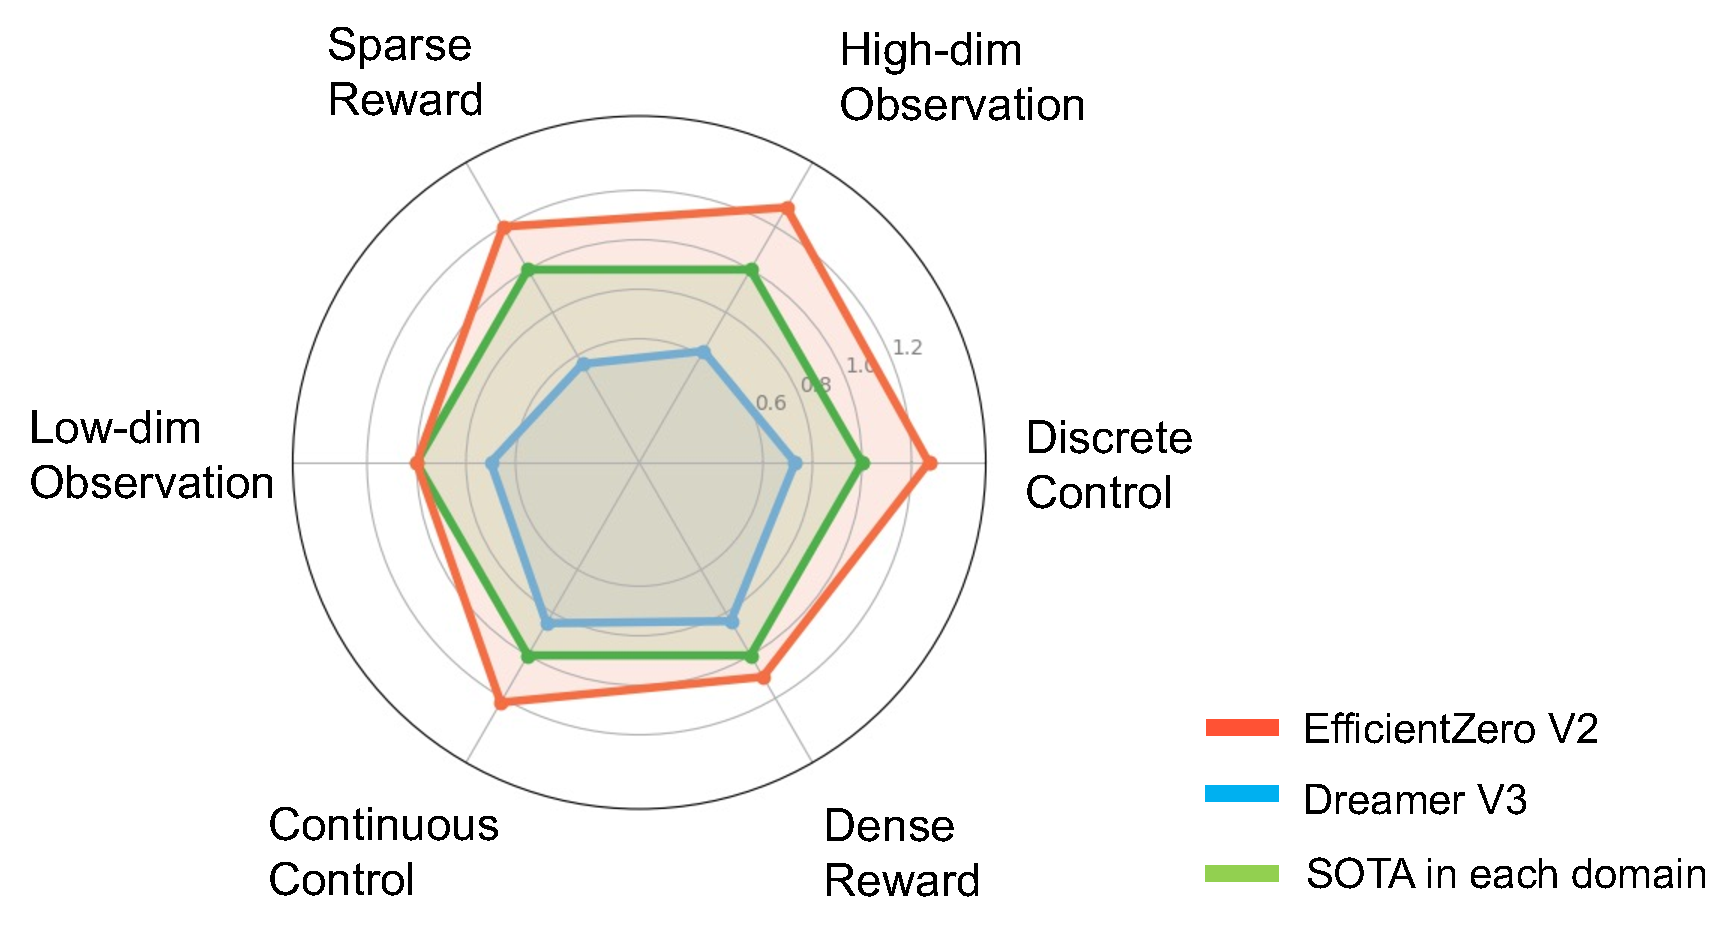
\includegraphics[width=0.47\textwidth]{sections/figs/concept.pdf}
\caption{Comparison between EfficientZero V2, DreamerV3 and other SOTAs in each domain. We evaluate them under the Atari 100k, DMControl Proprio, and DMControl Vision benchmarks. 
We then set the performance of the previous SOTA as 1, allowing us to derive normalized mean scores for both EfficientZero V2 and Dreamer V3. EfficientZero V2 surpasses or closely matches the previous SOTA in each domain.}
\label{main_sell}
\end{figure}

% For each metric, tasks aligning with the corresponding settings are selected. 


Previous studies have introduced a range of algorithms aimed at enhancing sample efficiency, including TD-MPC series \citep{hansen2022temporal, Anonymous2023TDMPC2}, EfficientZero \citep{ye2021mastering}, and the Dreamer series \citep{hafner2019dream, hafner2021mastering, hafner2023mastering}. Despite these advancements, these algorithms do not consistently attain superior sample efficiency across multiple domains. For example, TD-MPC \citep{hansen2022temporal} leverages Model Predictive Path Integral (MPPI) \citep{rubinstein1997optimization} control for planning. The huge computational burden in planning hinders its application in vision-based RL.
% \ywr{Emphasize TD-MPC fails in image-based RL}. 
EfficientZero \citep{ye2021mastering} employs the Monte-Carlo Tree Search (MCTS) algorithm, which masters discrete control. 
However, EfficientZero is unable to handle high-dimensional action spaces, especially in continuous control scenarios.
DreamerV3 \citep{hafner2023mastering} is a universal algorithm that extends to diverse tasks in a wide range of domains. However, as shown in Fig. \ref{main_sell}, DreamerV3 still has noticeable performance gaps to the state-of-the-art (SOTA) algorithms in each domain.
Thus, there remains an open question on how to achieve both high performance and sample efficiency across various domains at the same time. 
% This approach, however, poses challenges for EfficientZero in managing high-dimensional action spaces in continuous control scenarios.
% The lack of a general algorithm means that we require extra computational resources for choosing and tuning the algorithms when applying RL algorithm to a new application.
% \ywr{why this is a fundamental question?}


In this paper, we propose EfficientZero-v2 (EZ-V2), which can master tasks across various domains with superior sample efficiency.
EZ-V2 successfully extends EfficientZero's strong performance to continuous control, demonstrating strong adaptability for diverse control scenarios. 
The main contributions of this work are as follows. 
\begin{itemize}
    \item We propose a general framework for sample-efficient RL. Specifically, it achieves consistent sample efficiency for discrete and continuous control, as well as visual and low-dimensional inputs.
    % \ywr{be consistent.}
    \item We evaluate our method in multiple benchmarks, outperforming the previous SOTA algorithms under limited data. As shown in Fig.\ref{main_sell}, the performance of EZ-V2 exceeds DreamerV3, a universal algorithm, by a large margin covering multiple domains with a data budget of 50k to 200k interactions. 
    % \ywr{Do not use 's. such as the performance of EZ-V2.}
    \item We design two key algorithmic enhancements: a sampled-based tree search for action planning, ensuring policy improvement in continuous action spaces, and a search-based value estimation strategy to more efficiently utilize previously gathered data and mitigate off-policy issues.
\end{itemize}

% introduces two key algorithmic enhancements: a sampled-based tree search for action planning, ensuring policy improvement in continuous action spaces, and a search-based value estimation strategy to more efficiently utilize previously gathered data and mitigate off-policy issues.
% Our algorithm is built upon Efficient Zero, owing to the super-human performance of Efficient Zero in Atari 100k benchmark,
% Furthermore, the method reduces the number of simulations in tree search, which benefits the planning in large complex actions spaces. 
% Thus, EZ V2 is a universal RL algorithm that achieves state-of-the-art performance using limited data in both discrete and continuous action spaces and high-dimensional and low-dimensional observation spaces.
